%%%%%%%%%%%%%%%%%%%%%%%%%%%%%%%%%%%%%%%%%%%%%%%%%%%%%%%%%%%%%%%%%%%%
%%%%%%%%%%%%%%%%%%%%%%%%%% PREMIÈRE PARTIE %%%%%%%%%%%%%%%%%%%%%%%%%
%%%%%%%%%%%%%%%%%%%%%%%%%%%%%%%%%%%%%%%%%%%%%%%%%%%%%%%%%%%%%%%%%%%%

\part{Du document numérisé au \xmltei: nature du corpus, structure des documents et méthode de production des données}

Avant d'aborder la manière dont les catalogues sont manipulés de façon automatique, il importe de présenter ces documents. Dans cette partie sont donc présentés les catalogues comme typologie de documents, avant de décrire les catalogues de vente de manuscrits en particulier. C'est ensuite la manière dont les données sont produites qui est décrite, au travers d'une présentation du processus de transcription et de \gls{ocr}. À cette occasion est également présentée la structure des catalogues, ainsi que la manière dont celle-ci peut être utilisée pour modéliser les catalogues, afin de les encoder en \xmltei{}.

\chapter{Le marché des manuscrits autographes au prisme des catalogues de vente}
\chaptermark{Le marché des manuscrits autographes}
Ce chapitre présente l'objet d'étude du projet \mss{} : étudier le marché des manuscrits autographes du \scl{XIX}. parisien à partir de ses catalogues de vente et comprendre la construction du canon littéraire au prisme du marché du manuscrit.

\section{Pourquoi étudier le marché des manuscrits autographes et les catalogues de vente?}
\sectionmark{Pourquoi étudier le marché...}
\subsection{Qu'est-ce qu'un catalogue?}
Le catalogue est un objet d'étude ancien et une source importante pour les études littéraires et pour l'histoire de l'art. Il peut être défini comme un document présentant une collection et énumérant les items qu'elle contient, que cette collection soit celle d'une bibliothèque, d'un musée ou d'une personne privée. Selon l'historien de l'art Victor Stoichita, le catalogue fonctionne comme une organisation et une structuration d'une collection sous une forme textuelle, avec un travail classificatoire qui est le fruit d'une activité humaine. C'est un objet qui représente une collection sous la forme d'un discours. C'est pourquoi, pour Stoichita, le développement du catalogue est concomitant de celui de l'acte de collectionner lui-même\footcite[p. 119-124]{stoichita_instauration_1993}: cataloguer, c'est reconnaître le statut particulier d'une collection, à la fois ensemble d'objets et organisation intellectuelle de ceux-ci en fonction du goût du ou de la collectionneur.euse.

Au fil du temps, une collection est vouée à évoluer, avec l'acquisition, la vente ou la perte de différentes pièces. Elle peut aussi disparaître totalement, en étant détruite ou dilapidée. Les collections sont particulièrement sensibles aux évènements historiques, comme lorsque les possessions du clergé sont devenues des biens nationaux, avant d'être en partie vendues pour renflouer les caisses de l'État lors de la Révolution Française. En conservant l'image d'une collection à un moment donné, les catalogues sont donc des sources historiques importantes et ont fait l'objet de nombreuses recherches.

Mais avant d'expliquer à quelle fin les catalogues ont pu être utilisés, il peut être intéressant de commencer par dresser une typologie des différents types de catalogues existant, afin de mieux comprendre les objets qui sont étudiés par le projet \mssktb{}. Il importe tout d'abord de faire la différence entre le catalogue et son cousin, l'inventaire. L'inventaire, selon Victor Stoichita, se limite à énumérer les items d'une collection, sans nécessairement organiser ceux-ci. L'inventaire n'est pas un objet intellectuel, mais une simple liste; le système organisationnel suivi est conventionnel (ordre alphabétique, numéraire...). Pour Stoichita, la spécificité du catalogue se retrouve dans une définition de celui-ci qui date de 1690, écrite par La Furetière: un catalogue est une \enquote{liste \& mémoire qui contient plusieurs noms propres d'hommes, ou de livres disposez \textbf{selon un certain ordre}}\footcite[p. 122, le gras est ajouté par moi-même]{stoichita_instauration_1993}. C'est la dernière partie de la description qui exprime la spécificité de l'objet catalogue. Il suppose une organisation des informations qu'il contient, et donc la production d'un ordre qui lui est propre, et qui s'appuie sur les objets décrits pour produire un discours sur la collection.

Aujourd'hui, les catalogues peuvent être catégorisés sur la base d'une distinction disciplinaire. Il existe des catalogues de bibliothèques, contenant majoritairement des livres et des documents édités sur papier, et des catalogues de musées, qui eux sont plutôt consacrés aux unicums. À côté de ces deux types de catalogues se trouvent les inventaires de séries d'archives; ceux-ci, cependant, sont organisés selon l'entrée des pièces dans un fonds d'archives, et ne rentrent donc pas de la catégorie du catalogue. Mais la classification des catalogues peut aussi être faite sur des bases fonctionnelles, c'est-à-dire selon l'usage qui sera fait du catalogue. Dans ce cas, les catalogues de vente se distinguent des catalogues d'exposition, qui sont à distinguer des catalogues utilisés pour le fonctionnement d'une collection. Les derniers sont dédiés aux usager.ère.s d'une collection, que ce soient des employé.e.s d'une bibliothèque ou des lecteur.ice.s cherchant un ouvrage en particulier. Le catalogue sert ici de moyen de repérage au sein d'une collection. Les catalogues d'exposition, eux, ont à la fois le statut de publication scientifique et d'objets dérivés, supports du souvenir pour un public de touristes ou de visiteur.euse.s. Les catalogues de vente, enfin, se distinguent par leur fonction marchande, puisque leur rôle est d'aider à la vente des items qu'ils décrivent. Si, comme le dit Stoichita, un catalogue est consubstantiel à une collection, alors un catalogue de vente est consubstantiel à la dilapidation de celle-ci. Mais le catalogue est aussi le marqueur de la conscience qu'un.e collectionneur.e a de la spécificité de l'action de collectionner (et de vendre). Dans ce cas, le catalogue ne fait pas qu'exposer une collection, il porte aussi la marque de l'expert; les catalogues de vente sont des témoignages historiques de l'activité des commissaires priseurs et surtout des organisateurs de ventes.

Le catalogue fonctionne donc comme témoin d'une collection et d'une activité, celle de collectionner. Mais avec le développement des humanités numériques, les catalogues offrent de nouvelles possibilités, et c'est pourquoi ils sont l'objet de plusieurs initiatives. Contenant des descriptions d'items de façon souvent clairement structurée et compréhensible, ces documents peuvent en effet fonctionner comme des sortes de bases de données reflétant les contenus d'une collection. Contrairement à d'autres sources de données plus complexes (comme les textes littéraires), un catalogue encodé constitue une base de données \enquote{prête à l'emploi}, puisque les informations y sont structurées avec suffisamment de précision pour qu'il n'y ait pas besoin de mener une campagne d'extraction de données du texte. Il est alors possible de constituer des collections de catalogues, qui constituent des sources diachroniques et hautement homogènes sur un sujet. C'est de cette manière que sont utilisées les catalogues par le projet \href{https://bibale.irht.cnrs.fr/}{Bibale}, de l'Institut de recherche et d'histoire des textes (IRHT), projet visant à reconstituer des collections anciennes à l'aide de leurs catalogues. Les Archives nationales ont également réalisé des travaux sur les catalogues des bibliothèques ecclésiastiques saisies pendant la révolution; enfin, la bibliothèque Mazarine encode les inventaires des bibliothèques Mazarin et Richelieu en \xmltei{}\footcite[p. 8-9]{rondeau_du_noyer_encoder_2019}. 

\subsection{Catalogues et étude du marché}
Dans le cadre du projet \mssktb{}, ce sont des catalogues de vente de manuscrits autographes qui sont encodés automatiquement afin de constituer une base de données complète. Les catalogues sont ceux de ventes aux enchères et de revues spécialisées dans la commercialisation de manuscrits. Se pose cependant la question: sur quoi porte cette base de données? Au premier abord, il peut sembler que les catalogues de vente permettent de constituer une base de données sur les manuscrits, puisque ce sont de tels documents qui sont mentionnés dans les catalogues. Cependant, il serait erroné de se limiter à cette définition. En tant que base de données de manuscrits, les données du projet \ktb{} manquent en effet grandement d'exhaustivité: un nombre restreint de sources sont utilisées pour les catalogues. Plus largement, il est impossible de définir précisément un périmètre pour les manuscrits de la base de données: les autographes ne s'y trouvent pas à cause de caractéristiques qui leur sont intrinsèques (comme une origine géographique ou une date). Le corpus est constitué par le fait que les documents aient été commercialisés par certains vendeurs au \scl{XIX}. Dans ce cas, que dit cette base de données? C'est d'abord une base consacrée au marché des manuscrits au \scl{XIX}. C'est donc une base de documents autographes, mais perçus au prisme du marché de l'époque. Les informations contenues concernent donc moins les documents originaux qu'une perception historiquement située de ceux-ci. La base peut donc être utilisée comme un moyen pour étudier la constitution du canon littéraire; elle forme un objet d'étude pour l'histoire de la littérature.

La seconde question qui se pose est: qu'est-ce qui peut être fait avec une base de données de catalogues de vente? Ce mémoire se propose d'offrir une longue réponse à cette question, puisqu'il présente justement le développement d'outils numériques pour l'analyse et la diffusion de données issues de cette base. Plus brièvement, les catalogues de vente, en tant que regard sur le marché, sont des sources essentielles pour la recherche historique. L'analyse du marché de l'art est essentielle dans l'histoire de l'art, puisque le milieu de la vente est \enquote{l'un des fonctionnements des mondes de l'art}\footcite[p. 64]{de_maupeou_les_2013}. L'expression de \enquote{monde de l'art}, due au sociologue Howard S. Becker, est utilisée pour traduire l'idée que l'artiste n'est pas un.e créateur.ice isolé.e, mais une personne évoluant au travers de divers cercles et réseaux de sociabilités; la production artistique se situe alors dans une interaction, avec les attentes du public, avec la production faite par ses pairs artistes mais aussi avec le marché et un ensemble d'évènements sociaux, politiques et économiques qui adviennent en dehors du monde de l'art. La vente est donc constituante de la production artistique. Cette constatation est originaire de la sociologie des arts visuels, mais elle pourrait tout autant s'appliquer à la littérature. Dans ce contexte, les données contenues dans les catalogues de vente montre quel.le.s auteur.ice.s sont populaires sur le marché au \scl{XIX}, et illustrent donc les modèles et le canon qui sont en train de se constituer à l'époque. Ils permettent donc de développer une compréhension historique des sources de la littérature du \scl{XIX}. 

Peut-être parce que l'art s'apparente à un marché de luxe, où des objets uniques sont vendus pour une somme généralement élevée, les approches économiques sont particulièrement développées en histoire de l'art. C'est peut-être pour cela que les catalogues de vente y sont utilisés aussi régulièrement. Léa Saint-Raymond, par exemple, se sert de catalogues de ventes ayant eu lieu entre 1831 et 1925 pour étudier la pertinence du célèbre modèle \enquote{marchand-critique} dans le marché de l'art de l'époque\footcite{saint-raymond_revisiting_2019}. Ce modèle, développé par Cynthia et Harrison White, pose une modification qui aurait lieu dans le milieu de l'art parisien vers 1870-1880. Alors qu'avant, la valeur commerciale d'un.e artiste était directement un facteur de sa réussite institutionnelle (il fallait avoir obtenu son admission au Beaux Arts, être exposé au Salon), la décennie 1870 marque, selon les White, un changement de paradigme. Les institutions officielles perdent leur pouvoir de légitimation, et les nouveaux faiseurs de valeurs sont les marchands et les critiques d'art. Ce sont ces personnes qui seraient à même de faire la popularité d'une personne, et donc d'établir sa valeur financière. Cependant, grâce à une analyse des ventes de l'époque, Saint-Raymond montre que, jusque dans les années 1910, le salon reste l'élément déterminant dans la cote d'un artiste\footcite[p. 6-16]{saint-raymond_revisiting_2019}. Marchand.e.s et critiques, s'ils prennent de plus en plus de place dans le discours public sur l'art, ne gagneront donc une influence dans le marché que vingt à trente ans après la date mise en avant par Cynthia et Harrison White. Dans cette étude, le catalogue de vente est utilisé comme une source de données quantitatives, disponibles en grande quantité et sous une forme synthétique. En développant une approche quantitative de l'histoire de l'art, l'autrice remet en question des modèles développées en suivant une approche sociologique. Au sein du projet \mssktb{}, les catalogues sont perçus comme offrant les mêmes possibilités. Ces documents sont des sources synthétiques et structurées de données quantitatives. Ils peuvent être utilisés comme des outils dans une approche historique du marché de l'écrit au \scl{XIX}, d'abord, et ensuite pour une analyse du milieu et de la culture littéraire de l'époque, et donc pour analyser les sources de la culture littéraire contemporaine.


\section{La structure du corpus : périodisation, producteurs des documents et classification}
\sectionmark{La structure du corpus}
Le projet \mssktb{} existe maintenant depuis plusieurs années, pendant lesquelles les données utilisées ont continuellement été enrichies. Le projet dispose aujourd'hui d'une base de données faite de près de 500 catalogues, comprenant plus de 82000 entrées. Les catalogues proviennent de plusieurs sources différentes:

\begin{itemize}
	\item Une première série est composée de catalogues de ventes aux enchères. Celles-ci sont préparées par l'édition de catalogues listant les pièces qui seront vendues. Puisqu'il s'agit d'enchères, les prix ne sont bien sûr pas listés. Dans certains cas, les ventes sont thématiques: certaines sont par exemple consacrées à la révolution française ou aux campagnes napoléoniennes. Dans d'autres cas, les enchères sont consacrées à la vente d'une collection. Dans ce cas, c'est le nom du ou de la collectionneur.euse qui est donné à l'ensemble de la vente. Dans la plupart des cas, cependant, les ventes n'ont pas de thème particulier.
	\item Se trouve ensuite un premier périodique, le \textit{Catalogue de lettres autographes et manuscrits}. Celui-ci est édité par Antoine Laverdet, une des figures importantes du marché parisien des autographes, jusqu'en 1865. Le \textit{Catalogue} contient uniquement des entrées à prix fixes.
	\item Une autre revue d'autographes à prix fixes présente dans le corpus est la \textit{Librairie ancienne et autographes}, publiée par la famille Charavay. Cette famille, installée à Paris et à Lyon, est un acteur important dans le marché du manuscrit parisien. La famille possède une librairie et édite plusieurs revues consacrées aux autographes. En 1865, Gabriel Charavay rachète le cabinet d'autographes d'Auguste Laverdet\footcite[p. 18-21]{rondeau_du_noyer_encoder_2019} lorsque celui-ci prend sa retraite\footcite[p. 3]{gabay_selling_2020}. En plus de publier des revues et de posséder une librairie, la famille Charavay, et surtout Étienne, chartiste de formation, organise de nombreuses ventes aux enchères
	\item Enfin se trouve la publication mensuelle \textit{Revue des Autographes, des curiosités de l’histoire et de la biographie}, qui liste des items en vente à prix fixe. Cette revue est également éditée par la famille Charavay. Elle se distingue des autres publications, tout d'abord par sa durée de publication, puisqu'elle est éditée entre 1866 et 1936. Ensuite, cette revue n'est pas seulement dédiée à la vente: elle contient également des articles complets sur les manuscrits. Au fil du temps, la part d'articles diminue dans cette revue, et au final ne subsistent dans la revue que des quelques actualités et des listes d'items dans le fonds de la librairie Charavay qui sont en vente\footcite[p. 3]{gabay_selling_2020}. La part \enquote{catalogue de vente} de la revue augmente donc avec le temps.
\end{itemize}

Le corpus composé à partir de l'encodage de ces différentes sources couvre une période chronologique qui commence vers 1840; les données disponibles après 1905 sont bien plus rares, bien que des données soient disponibles jusqu'à plus tard (figure \ref{fig:countitm}). Le nombre d'items mis en vente par an évolue régulièrement à partir de 1840, pour connaître une apogée de 1880 au milieu des années 1895, où entre 1500 et plus de 3500 items sont mis en vente annuellement. Ces items sont en très grande majorité des manuscrits vendus à pris fixes; le marché des enchères d'autographes, tel qu'il est représenté dans le corpus de catalogues, est relativement irrégulier, puisque presque aucun manuscrit n'est mis en vente aux enchères certaines années, alors que, pour l'année 1888, 3714 manuscrits sont vendus aux enchères, pour seulement 1414 pièces vendues à prix fixe. À partir de 1895, le nombre de manuscrits mis en vente décline vite, et les ventes après 1900 se font très rares (à l'exception de quelques années où ont lieu de nombreuses ventes aux enchères) (figure \ref{fig:countitm}). Comment interpréter cette courbe en cloche de l'évolution du nombre de manuscrits vendus? Il est bien sûr possible que le marché connaisse un essor rapide après 1860 (ce qui correspond à la mise en publication de la \textit{Revue des autographes}), pour péricliter au tournant du siècle. Il me semble cependant plus probable que l'évolution décrite ici reflète surtout les données disponibles par le projet \mssktb{}. En effet, si l'on compare le marché du manuscrit aux beaux-arts, la différence est frappante. Selon une analyse de Saint-Raymond et de Maupéou des marchands d'art présents dans le Bottin, le marché de tableaux connaît une expansion régulière à partir de 1815, même si la situation commence à se stabiliser à partir de 1852, avec un taux de renouvellement des marchands d'environ 12\% par an\footcite[p. 67-68, 75]{de_maupeou_les_2013}. Cependant, le marché ne décline pas du tout après 1890, au contraire. À cette date se développe un marché concurrentiel, mais qui est en permanente expansion: l'écroulement du marché de tableaux n'aura lieu qu'en 1931\footcite[p. 67-68]{de_maupeou_les_2013}. Il est relativement probable que le marché des manuscrits ait suivi une courbe d'évolution semblable, et qu'il ne se soit pas écroulé de façon aussi brutale que les données visibles en \ref{fig:countitm} le laissent présumer. 

\begin{figure}[h]
	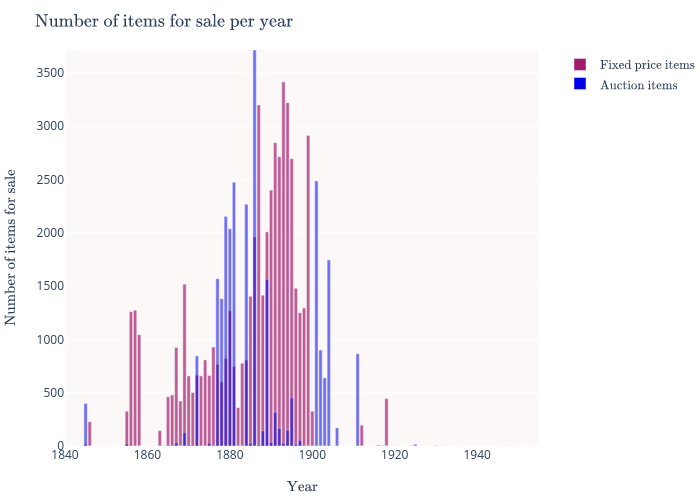
\includegraphics[width=\textwidth]{annexes/fig_count_itm.png}
	\caption{Nombre d'items à prix fixes et aux enchères mis en vente par an (en francs constants 1900)}
	\label{fig:countitm}
\end{figure}

C'est également ce que l'évolution des prix laisse présumer (figure \ref{fig:meditm}). En effet, le prix médian d'un item par an connaît une croissance exponentielle. En 1856, ce prix est de 3,06 francs\footnote{Tous les prix sont exprimés en francs constants au taux de 1900.}. En 1865, dix ans plus tard, le prix médian est de 4,08 francs. L'évolution continue d'être d'environ un franc par an dans la décennie 1865-1855, puisque le prix médian d'un item est de 5,10 francs en 1875. C'est au cours de la décennie 1875-1885 que les prix explosent, puisque le prix médian d'un manuscrit double pour atteindre 10,20 francs en 1885, avec des pics à 15,30 et 15,60 francs les années 1882 et 1891. Ce niveau se maintient à peu près jusqu'à l'année 1900, après laquelle très peu de données sont disponibles. Les catalogues reflètent donc une évolution constante des prix, avec un pic au alentours des années 1880-1900. En plus de cette évolution des prix, il semble y avoir lieu une explosion du prix des items les plus chers. En effet, à partir des années 1880, le prix moyen pour un item est systématiquement supérieur au prix médian (un graphique pour les prix moyens est visible en annexes: \ref{appendix:avgitm}). En 1891, le prix moyen pour un item atteint les 20 francs. Il est également à remarquer que le troisième quartile, c'est-à-dire le prix au dessous duquel 75\% des items sont vendus, augmente grandement à partir des années 1880, et s'éloigne du prix médian (comme cela apparaît dans un graphique visible en annexes: \ref{appendix:quartitm}). Si les données se font rares après 1900, il semblerait que les prix des manuscrits mis en vente continuent à augmenter. Ces courbes de prix sont autant d'arguments supplémentaires pour supposer que le marché du manuscrit ne s'effondre pas au tournant du siècle: à cette date, les prix atteignent des niveaux encore inégalés. Bien après 1900, la tendance haussière du marché semble se maintenir. En 1919, le prix médian d'un item est de 45 francs et le prix moyen de 189,91 francs; en 1927, le prix médian est de 163 francs et le prix moyen est de 293,25 francs. Ces nombres sont partiellement imputables au taux d'inflation, qui est très stable jusqu'à 1900 avant d'augmenter, et surtout à partir de la première guerre mondiale\footcite{piketty_les_2001}. Cependant, ces prix corroborent l'idée que le marché ne s'effondre pas après 1900, contrairement à ce que les données laissent supposer.

\begin{figure}[!h]
	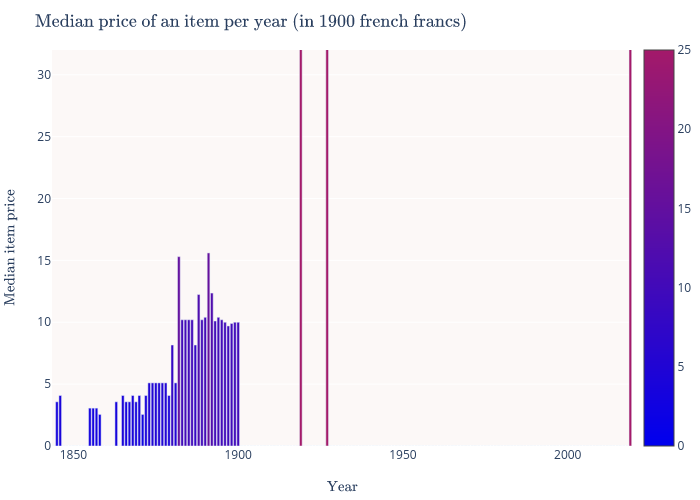
\includegraphics[width=\textwidth]{annexes/fig_med_itm.png}
	\caption{Prix médian d'un item par an (en francs constants 1900)}
	\label{fig:meditm}
\end{figure}

Au sein d'un même catalogue, la distribution des prix est toujours semblable, comme le montre la figure \ref{fig:violin}. La grande majorité des catalogues est composée d'éléments peu coûteux (souvent moins de dix francs le manuscrit). De façon peut-être surprenante, le faible prix d'un manuscrit n'implique pas nécessairement que l'auteur.ice soit une personne peu célèbre. Par exemple, dans la 165\up{e} \textit{Revue des autographes...}, un manuscrit de John-Quincy Adams, président américain, est vendu cinq francs. Malgré une majorité de prix faibles, il y a une très grande plage de prix dans les catalogues, puisqu'une poignée de manuscrits sont vendus à des prix extrêmement élevés, près d'une centaine de fois plus cher que les autres. Ces manuscrits sont régulièrement le fait de personnes célèbres. Dans le numéro 165 de la \textit{Revue des arts...}, par exemple, parmi les dix manuscrits les plus chers se trouvent des documents attribués à Fénelon, Rousseau, Robespierre et Elisabeth I reine du Royaume-Uni.

\begin{figure}[p]
	\centering
	\begin{subfigure}{0.6\textwidth}
		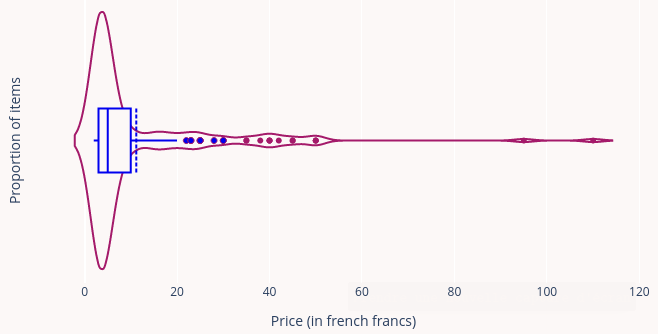
\includegraphics[width=\textwidth]{img/rda70_distrib.png}
		\caption{\textit{Revue des autographes...}, n°70, Novembre 1881, publiée par Eugène Charavay}
	\end{subfigure}
	\begin{subfigure}{0.6\textwidth}
		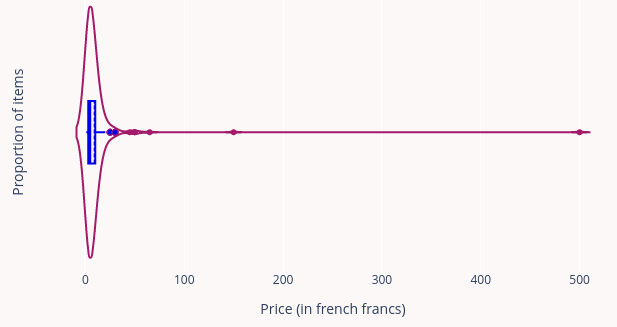
\includegraphics[width=\textwidth]{img/rda100_distrib.png}
		\caption{\textit{Revue des autographes...}, n°100, Octobre 1886, publiée par Eugène Charavay}
	\end{subfigure}
	\begin{subfigure}{0.6\textwidth}
		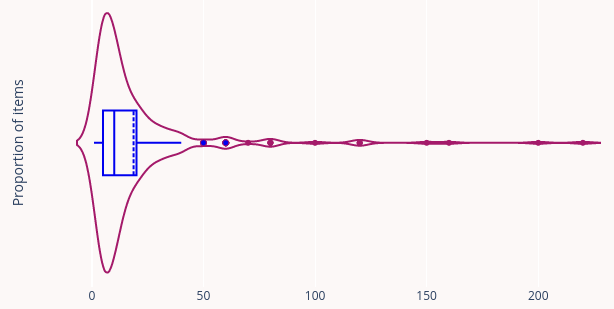
\includegraphics[width=\textwidth]{img/rda165_distrib.png}
		\caption{\textit{Revue des autographes...}, n°165, Avril 1894, publiée Mme Charavay}
		\label{fig:rda165}
	\end{subfigure}
	\begin{subfigure}{0.6\textwidth}
		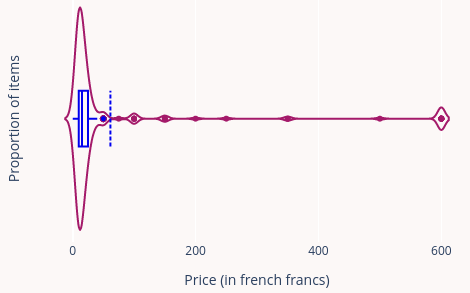
\includegraphics[width=\textwidth]{img/lad507_distrib.png}
		\caption{\textit{Lettres autographes et documents historiques}, n°507, avril 1919, publiée par Noël Charavay}
	\end{subfigure}
	\caption{Distribution des prix au sein d'un même catalogue (en francs courants)}
	\label{fig:violin}
\end{figure}

Après avoir fait cette présentation du corpus de catalogues \enquote{dans l'abstrait}, il est maintenant temps de voir comment les catalogues et les entrées sont organisées, et comment cette organisation peut servrir de modèle afin de concevoir une représentation en \xmltei{} de ces documents.

\chapter{Production des données: de l'OCR à la \tei{}}
\chaptermark{Production des données}
Au sein du projet \mssktb{}, la première manière d'étudier les catalogues de vente est de les encoder numériquement. Cet encodage naît d'une nécessité technique: les imprimés en tant que tels peuvent être analysés par une personne humaine, mais ne sont pas manipulables par une machine. Il est donc nécessaire d'extraire le texte des catalogues. Ce texte extrait, afin d'être manipulable par une machine, doit être ensuite conservé dans un format structuré et hiérarchisé, qui permette d'accéder facilement aux différentes entrées de catalogue, et aux différentes parties de ces entrées. Avant de pouvoir manipuler et analyser le texte, il est donc nécessaire de l'extraire, de le modéliser et de l'encoder en un format qui permette la mise au point de méthodes computationnelles. Cet encodage est le fruit d'une sélection et d'une interprétation des informations contenues dans les catalogues: certaines caractéristiques de ceux-ci sont privilégiées et d'autres sont abandonnées afin de parvenir à une édition numérique qui soit manipulable par une machine.

\section{Extraire le texte des imprimés: la transcription des catalogues}
\sectionmark{Extraire le texte des imprimés}
Après avoir présenté le processus d'encodage en général, cette section décrit la structure des catalogues au niveau du document complet, de la page et de l'entrée ainsi que la manière dont les pages de catalogues sont segmentées en utilisant \textit{SegmOnto}. Cet intérêt pour la structure des catalogues est essentiel, puisque c'est cette structure qui permet de les modéliser, et donc de préparer leur édition en \xmltei{}.

\subsection{Une chaîne de traitement pour la transcription du texte}
L'extraction du texte des catalogues repose fortement sur \textit{eScriptorium}, une application en ligne de transcription\footcite{stokes_escriptorium_2021}. Elle permet la transcription manuelle ou automatisée de documents et est particulièrement utilisée pour entraîner des modèles d'\gls{ocr}. En effet, l'entraînement d'un tel modèle se fait en produisant de la vérité de terrain, c'est-à-dire des documents transcrits à la main grâce auxquels le modèle pourra \enquote{apprendre} à reconnaître des caractères. L'application offre une interface graphique (visible en annexes: \ref{appendix:escriptorium}) et s'appuie sur \textit{Kraken}, un moteur de reconnaissance optique de caractères qui supporte un très grand nombre d'alphabets (latin, grec, arabe...). \textit{eScriptorium} est développé depuis 2018 à l'EPHE comme remplacement à \textit{Transkribus}. Cette seconde plateforme de transcription a un fonctionnement analogue, mais est entièrement propriétaire. Non seulement le code source de l'application et de son moteur d'\gls{ocr} ne sont pas accessibles, mais les modèles entraînés par les utilisateur.ice.s de \textit{Transkribus} ne peuvent être accédés directement. Cela rend impossible l'utilisation d'un tel modèle en dehors de l'application. En utilisant \textit{eScriptorium}, au contraire, l'extraction du texte des catalogues a un double intérêt: tout d'abord, elle permet de produire des données à traiter; ensuite, elle permet de produire des modèles d'\gls{ocr} qui sont réutilisables, soit sur d'autres applications, soit en utilisant directement \textit{Kraken}, et qui peuvent être partagés et réutilisés par d'autres chercheur.euse.s.

L'extraction du texte est faite de façon semi-automatisée: une étape automatique de transcription est suivie d'une correction manuelle. Dans un premier temps, le texte est extrait automatiquement des catalogues grâce à un modèle d'\gls{ocr} pour les imprimés de l'époque contemporaine. Celui-ci est développé depuis des années, notamment à partir des catalogues de vente de manuscrits du projet \ktb{}\footcite[p. 34-35]{janes_du_2021}. Une fois ce texte extrait, une phase de correction manuelle des données est nécessaire: puisque les entrées de catalogue sont retraitées et diffusées sur un site internet, elles ne doivent pas contenir d'erreurs. Dans un premier temps, les différentes zones de texte doivent être définies. Cette segmentation de la page en différentes parties est entreprise par défaut par \textit{eScriptorium}. Cependant, la segmentation de cette application unifie les zones de texte dans des polygones, sans distinguer les différences ou hiérarchies qui peuvent exister dans une zone de texte, comme cela apparaît dans l'exemple \ref{fig:seg}. La segmentation de la page est donc refaite manuellement, en utilisant le vocabulaire \textit{SegmOnto}, comme cela est décrit plus bas. Il faut ensuite corriger les données elles-mêmes, c'est-à-dire reprendre manuellement la transcription afin de s'assurer qu'elle corresponde au texte. Une fois que les catalogues ont été transcrits, cette transcription est exportée en \alto{}. Ce format \xml{} reproduit la structure physique d'un document en associant à chaque ligne de texte sa position sur la page en pixels. Ce format est ensuite transformé pour produire des fichiers \xmltei{}, un format qui permet l'encodage d'un catalogue entier. La \tei{} permet, comme cela est expliqué plus tard, un encodage sémantique d'un document entier, et non la relation entre le texte et le document dont il est transcrit. Dans le projet \mssktb{}, la conversion de l'\alto{} en \tei{} était originellement faite grâce à \textit{GROBID-Dictionnaries}, un outil produisant des fichiers \tei{} sur mesure pour des catalogues\footcite{khemakhem_automatically_2018}. Cet outil, basé sur l'intelligence machine, n'est plus en usage par le projet; il est en train d'être remplacé par des méthodes plus simples, basées sur la détection de motifs dans le texte.

\begin{figure}[h]
	\centering
	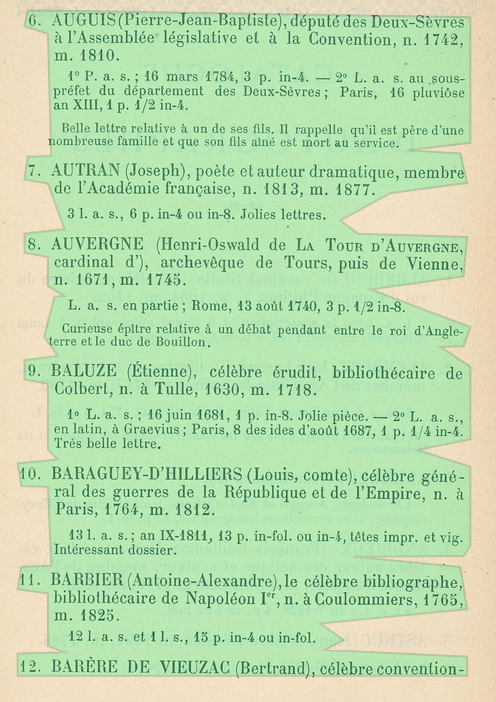
\includegraphics[width=0.4\textwidth]{img/cat_000445_p2}
	\caption{Exemple de segmentation automatique par \textit{eScriptorium}}
	\label{fig:seg}
\end{figure}


\subsection{Comprendre la structure du document pour préparer l'édition numérique}
L'encodage numérique d'un document se doit, autant que possible, d'être représentatif du document originel ou de certains aspects de celui-ci qui sont considérés comme importants en fonction des objectifs scientifiques du projet. La première étape de l'encodage est donc de comprendre la structure de ce qui sera encodé. Comme cela a été dit, plusieurs typologies de documents existent; dans le cadre de mon stage, la production de données s'est concentrée sur les catalogues de ventes aux enchères organisées par Étienne Charavay. C'est donc à partir de la structure de ceux-ci que s'appuie la présentation qui suit.

\subsubsection{La structure des catalogues}
L'encodage numérique repose sur des choix scientifiques: il n'est pas possible d'encoder toutes les caractéristiques possibles d'un document. Il est donc nécessaire de faire des choix qui privilégient les enjeux scientifiques du projet; ces choix se reflètent dans ce qui est conservé et ce qui ne l'est pas au sein  des documents. Le projet \mssktb{} choisit une orientation particulière, qui se concentre sur les manuscrits en vente dans les catalogues\footcite[p. 27]{rondeau_du_noyer_encoder_2019}. Cela implique donc que certaines pages de catalogues ne sont pas retranscrites ni encodées. Seulement une page de catalogue de vente aux enchères sur deux transcrite, puisque seulement une page sur deux est imprimée: l'autre page est quadrillée, et utilisée par le commissaire priseur pour tenir le compte des ventes: en face de chaque item vendu est écrit le prix de vente ainsi que le nom de l'acheteur.euse. Dans les revues-catalogues à prix marqués, les pages contenant des articles et des réclames ne sont pas retranscrites. D'abord, leur retranscription ne servirait pas les objectifs du projet. Mais de plus, ces pages, qui contiennent des images, sont trop homogènes pour le processus de reconnaissance optique de caractères. En effet, un tel processus repose sur l'entraînement d'un logiciel qui \enquote{apprend} à reconnaître des caractères dans un texte numérisé. Ce logiciel ne pouvant par défaut pas faire la distinction entre le texte et les parties graphiques des catalogues, il cherche à interpréter les illustrations comme du texte. Il est donc important de faire la différence entre la structure du document réel, tel qu'il est conservé par une bibliothèque, et la structure retenue pour ce projet, qui ne contient que les pages de catalogue considérées comme étant utiles. La page de titre d'un catalogue est retenue pour deux raisons: elle permet d'identifier celui-ci et offre des données bruitées (puisque cette page contient des motifs graphiques), qui sont utiles pour entraîner le logiciel de reconnaissance de caractères. Les catalogues de vente aux enchères contiennent également une ou deux pages introductives (qui présentent la vente et d'autres ouvrages publiés par l'éditeur). Celles-ci sont transcrites, là encore pour produire des données bruitées. Les pages de conclusion (qui contiennent notamment une liste de publications de l'éditeur) ne sont pas retranscrites. Le corps d'un catalogue est fait de pages listant les manuscrits en vente. Ces pages sont la source des données utilisées par \mssktb{}, et sont donc décrites ci-dessous.

Comme cela apparaît dans la figure \ref{fig:catpage}, la structure des pages de catalogues présente une grande régularité. La page de gauche présentée ici fait partie des quelques pages \enquote{spéciales} qui sont contenues dans les catalogues, puisque c'est la première page listant les items en vente. Elle débute donc par un bandeau décoratif et un titre dans une police plus grande que celle utilisée dans le reste de la page. Les autres pages listant des pièces en vente ont une structure plus homogène, puisqu'elles ne contiennent ni d'éléments graphiques ni de différence dans les fontes utilisées. La structure de la majorité des pages de catalogues ressemble donc à la page de droite dans la figure \ref{fig:catpage}. Les entrées se succèdent les unes après les autres; chaque entrée de catalogue étant numérotée, le début d'une nouvelle entrée est facilement identifiable grâce à son identifiant numéraire.

\begin{figure}[h]
	\centering
	\begin{subfigure}{0.49\textwidth}
		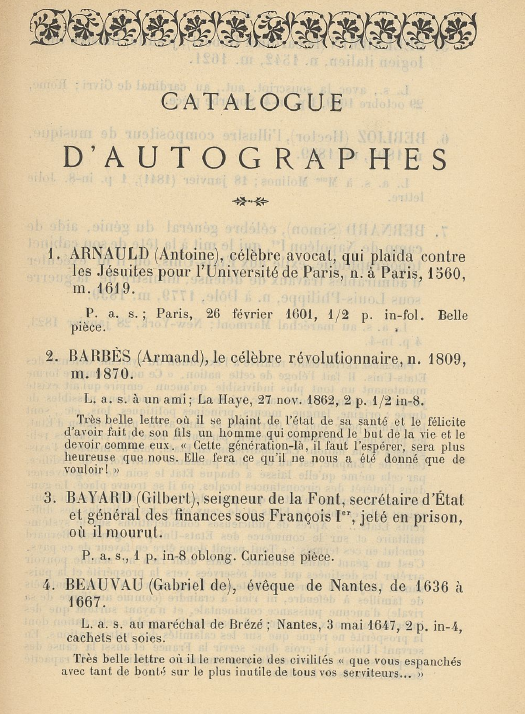
\includegraphics[width=\textwidth]{img/CAT_000441_0.png}
	\end{subfigure}
	\begin{subfigure}{0.49\textwidth}
		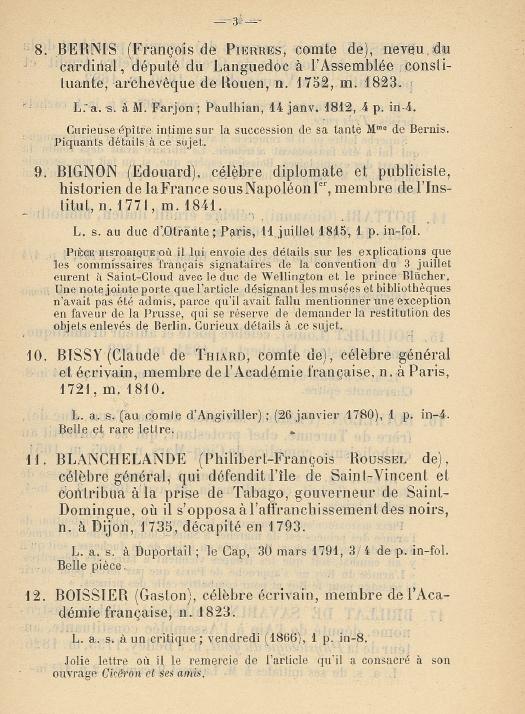
\includegraphics[width=\textwidth]{img/CAT_000441_1.png}
	\end{subfigure}
	\caption{Deux pages de catalogues de ventes aux enchères (\textit{Catalogue d'une précieuse collection de lettre autographes}, vente Étienne Charavay, 20 mai 1890)}
	\label{fig:catpage}
\end{figure}

\subsubsection{Appréhender la structure de la page à l'aide de SegmOnto}
La segmentation de la page en zones est une tâche centrale dans la transcription de documents. Elle est définie par Antonacopoulos et al. (2011, cité.e.s par Thibault Clérice\footcite[p. 4]{clerice_you_2022}) comme l'identification de zones de textes sur une page et la classification de ces zones en fonction de leur contenus. L'analyse de la disposition des informations sur une page est une étape importante dans tout processus de lecture, puisque c'est ainsi qu'un.e lecteur.ice aborde un document\footcite{christensen_segmonto_2022}. La segmentation a tout d'abord une utilité \enquote{intellectuelle}: elle permet de mieux comprendre comment les contenus d'un document s'organisent sur une page. Ce processus a également un rôle essentiel pour l'automatisation de la transcription automatique: la détection des zones de texte est une étape préalable à la reconnaissance des caractères. De plus, expliciter la distinction entre les différentes parties de la page permet, ultérieurement, de filtrer les différentes parties du texte pour ne conserver que celles qui sont pertinentes. Cela est particulièrement utile pour la reconnaissance optique de caractères. Si un document contient dans sa partie centrale de l'imprimé et dans ses marges du texte manuscrit et que les deux parties sont transcrites, l'entraînement d'un modèle sur ce document aura des résultats pour le moins problématiques. Le modèle apprendra en effet à identifier deux formes d'écritures très différentes comme étant la même. C'est ici que le zonage du texte est pertinent: il permet, par exemple, de ne conserver que le texte principal, et donc de diminuer le bruit présent dans les données.

La segmentation des zones faite automatiquement par \textit{Kraken} est reconnue comme étant une faiblesse de ce moteur d'\gls{ocr}\footcite[p. 1]{clerice_you_2022}. Celle-ci se base sur la construction d'un ou de plusieurs polygones pour englober le texte d'une page (figure \ref{fig:seg}). Ce système permet de définir une zone sur laquelle extraire du texte; cependant, il ne perçoit pas la fonction des différents éléments d'une page, et ne peut les considérer comme des éléments ayant une valeur différente. Par conséquent, Kraken a tendance à agglomérer dans un seul polygone des zones de texte qui devraient être considérées de façon distinctes. C'est le cas dans l'exemple \ref{fig:seg}, où tout le corps de la page est intégré dans une seule zone de texte. La segmentation faite par Kraken ne correspond donc pas aux besoins de la production de vérité de terrain réutilisable. Aussi doit-elle être remplacée. Des méthodes alternatives ont été développées pour une annotation sémantique des documents qui soit plus qualitative, comme \textit{YALTAi}\footcite{clerice_you_2022}, qui s'appuie sur des méthodes de reconnaissance des formes. Cet outil n'était pas encore fonctionnel lors de la phase de transcription de documents de mon stage; aussi la segmentation des catalogues a-t-elle été faite manuellement.

Segmenter un texte manuellement n'est pas difficile; la classification des zones, cependant, ne peut être faite en utilisant un vocabulaire \enquote{fait maison}: une vérité de terrain n'est réutilisable par d'autres que si le texte retranscrit est segmenté de façon compréhensible. Dans un souci d'interopérabilité, la définition de zones dans la page a donc été fait à l'aide de \textit{SegmOnto}, une ontologie pour la segmentation de documents\footcite{christensen_segmonto_2022, gabay_segmonto_2021}. Utiliser un vocabulaire commun à plusieurs projets est un moyen de rendre les données produites plus facilement compréhensibles par d'autres et de faciliter leur réutilisation par différents projets de recherche. \textit{SegmOnto} définit un vocabulaire permettant une segmentation sémantique des document, c'est-à-dire un découpage qui explicite le rôle des différentes parties de la page. Le projet a développé une approche matérielle des documents\footcite{gabay_segmonto_2021} qui cherche à définir un vocabulaire commun et simple pour segmenter la plus grande quantité de manuscrits possibles. Ce vocabulaire est conçu de façon modulaire: chaque polygone définissant une zone doit être annoté avec un terme (dit \enquote{type}) issu d'un vocabulaire contrôlé défini par \textit{SegmOnto}; l'un de ces termes est \enquote{CustomZone}, qui permet de définir des zones n'appartenant pas à \textit{SegmOnto}. Ces différents types peuvent de plus être précisés grâce à des sous-types (qui sont librement définis par un projet); enfin, les zones peuvent être hiérarchisées entre elles. Une zone conforme à \textit{SegmOnto} doit donc correspondre à l'expression suivante: \texttt{type(:sous-type)?(\#\textbackslash{}d)?} (soit un type suivi d'un sous-type optionnel et d'une hiérarchisation optionnelle).

\textit{SegmOnto} définit les zones à l'aide d'un vocabulaire simple à la finalité pratique: pouvoir filtrer les différentes parties d'une page pour entraîner des modèles d'\gls{ocr} sur des données propres. Par conséquent, l'utilisation de \textit{SegmOnto} pour structurer des catalogues de vente de manuscrits est elle aussi simple. Les éléments utilisés par \ktb{} sont les suivants:

\begin{itemize}
	\item \texttt{MainZone}: cet zone correspond à la partie principale d'une page.
	\item \texttt{TitlePageZone}: cette zone identifie la partie principale d'une page de titre. Elle est utilisée à la place de \texttt{MainZone} car la page de titre contient de nombreux éléments graphiques, alors que la partie principale des autres pages n'en contient pas. Il est donc important de faire la différence entre ces deux types de pages afin de pouvoir filtrer le bruit qui peut être présent dans les données.
	\item \texttt{GraphicZone}: cette zone permet de contenir des éléments graphiques qui doivent être distingués du corps du texte.
	\item \texttt{RunningTitleZone} est une zone permettant d'indiquer la présence d'un titre courant.
	\item \texttt{MarginTextZone}: l'usage de cette zone permet de contenir des signatures et autres notes manuscrites en marge du texte.
	\item \texttt{CustomZone:Entry} est une zone propre au projet \mssktb{} qui permet de désigner une entrée de catalogue.
	\item \texttt{CustomZone:EntryEnd} est utilisée lorsqu'une entrée de catalogue se poursuit sur plus d'une page: elle sert à indiquer qu'une entrée a été débutée à la fin de la page précédente.
\end{itemize}

À l'aide de ces sept éléments (dont deux qui n'ont pas été définis par \textit{SegmOnto}), il est possible d'annoter l'intégralité des catalogues. Comme cela apparaît dans les exemples \ref{fig:catzones}, les éléments utilisés diffèrent beaucoup en fonction de la page qui est traitée. Les pages contenant des items en vente (\ref{fig:catp1}, \ref{fig:catp2}) sont majoritairement composées d'une \texttt{MainZone} contenant des \texttt{CustomZone:Entry} et \texttt{CustomZone:EntryEnd}. La première de ces deux pages est également la première page du catalogue, et elle contient donc également une \texttt{RunningTitleZone} contenant le titre courant, ainsi qu'une \texttt{GraphicZone} pour inclure un bandeau graphique. La segmentation de la page de titre (\ref{fig:cattitle}) diffère beaucoup des autres pages du catalogue. La page de titre contient beaucoup d'éléments graphiques; pour la distinguer des autres pages, elle est donc contenue dans une \texttt{TitlePageZone}. Elle peut également être complétée de signatures, ou de notes manuscrits; ici, une signature est contenue dans un \texttt{MarginTextZone}.

\begin{sidewaysfigure}[p]
	\begin{subfigure}{0.33\textwidth}
		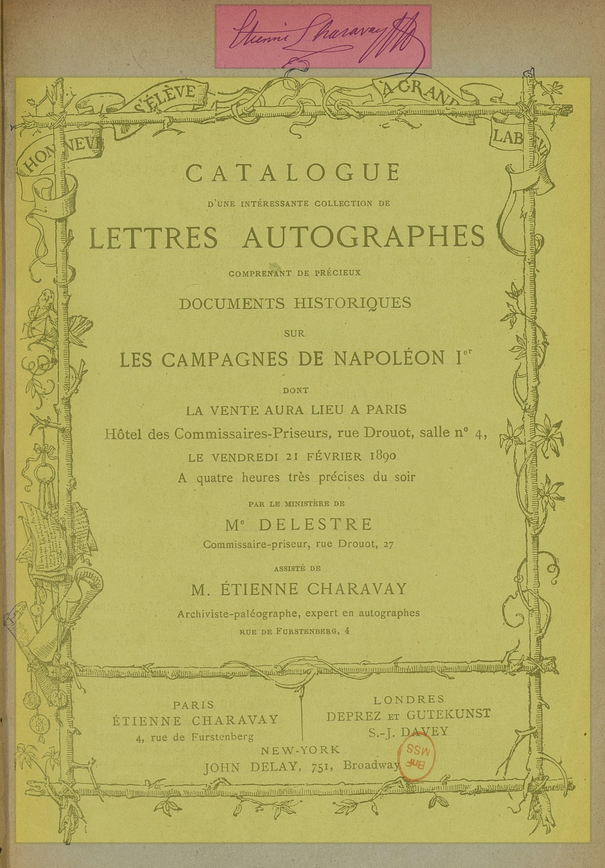
\includegraphics[width=\textwidth]{img/cat_000434_couv_zones.png}
		\caption{La page de titre}
		\label{fig:cattitle}
	\end{subfigure}
	\begin{subfigure}{0.33\textwidth}
		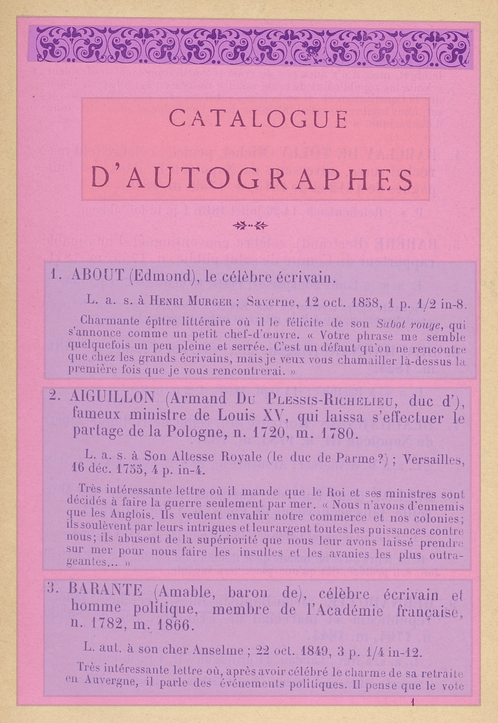
\includegraphics[width=\textwidth]{img/cat_000434_p1_zones.png}
		\caption{La première page du catalogue}
		\label{fig:catp1}
	\end{subfigure}
	\begin{subfigure}{0.33\textwidth}
		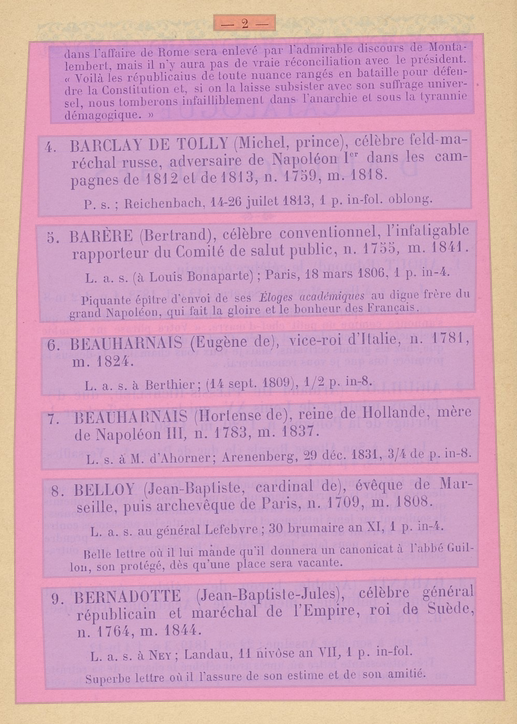
\includegraphics[width=\textwidth]{img/cat_000434_p2_zones.png}
		\caption{La seconde page du catalogue}
		\label{fig:catp2}
	\end{subfigure}
	\caption{La segmentation de trois pages de catalogues de ventes aux enchères (\textit{Catalogue d'une précieuse collection de lettre autographes}, vente Étienne Charavay, 21 février 1890)}
	\label{fig:catzones}
\end{sidewaysfigure}

Si cette segmentation n'est pas réutilisée dans une fois que les fichiers \alto{} ont été convertis en \tei{}, cette étape est néanmoins importante. D'abord, elle garantit que les données produites par \mssktb{} soit réutilisable par d'autres projets, puisque l'utilisation de \textit{SegmOnto} facilite la diffusion de vérité de terrain. Ensuite, le découpage des pages de catalogues en zones met en avant une unité intellectuelle pour les catalogues: celle des items vendus. Mettre en avant l'item comme élément structurant marque un éloignement des catalogues papiers, où c'est la page qui joue un rôle d'importance. Au contraire, les catalogues encodés ne gardent pas mention des pages, mais prennent pour élément central les entrées individuelles.


\subsubsection{Description des entrées de catalogue: préparer l'édition \tei{}}
La régularité présente au niveau du catalogue complet se retrouve également au niveau des entrées: chaque item en vente est décrit de façon analogue à ce qui est visible en \ref{fig:catitem}. Après le numéro de l'item se trouve le nom de l'auteur.ice du manuscrit ainsi qu'une description succincte de cette personne. Il arrive que, à la place du nom de l'auteur soit utilisé une titre comme \enquote{Documents divers} ou la mention d'un évènement historique (\enquote{Révolution française}). Lorsque c'est avec le nom d'une personne que débute une entrée de catalogue, celui-ci est souvent composé d'un nom de famille complet ainsi que d'un prénom, abrégé ou non. Celui-ci est souvent entre parenthèses et après le nom de famille. La description mentionne quelques faits biographiques. Dans la grande majorité des cas, ceux-ci se concentrent sur l'occupation de la personne, sa date de naissance et de décès; parfois, la façon dont une personne est morte peut également être décrite. Ensuite se trouve une description de l'item en vente lui-même (\enquote{L. a. s. au citoyen Victor Delaunay...}). Cette description, pour des raisons d'économie d'espace, s'appuie sur un vocabulaire et une structure très codifiée, avec de nombreuses abréviations. D'abord est indiqué le type de lettre (\enquote{L. a. s.}, pour \enquote{Lettre autographe signée}). Dans le cas d'une lettre est également indiqué le ou la destinataire ainsi que le lieu et la date où celle-ci a été écrite. Après cette description très succincte et normée se trouve parfois un paragraphe additionnel donnant des détails sur les manuscrits, comme c'est le cas dans cet exemple. C'est en général dans ce paragraphe qu'est indiqué le sujet du document en vente, ainsi que, parfois, un extrait de celui-ci. Lorsqu'un manuscrit est vendu à prix fixe, alors ce prix est également indiqué à la fin de l'entrée.

\begin{figure}[h]
	\centering
	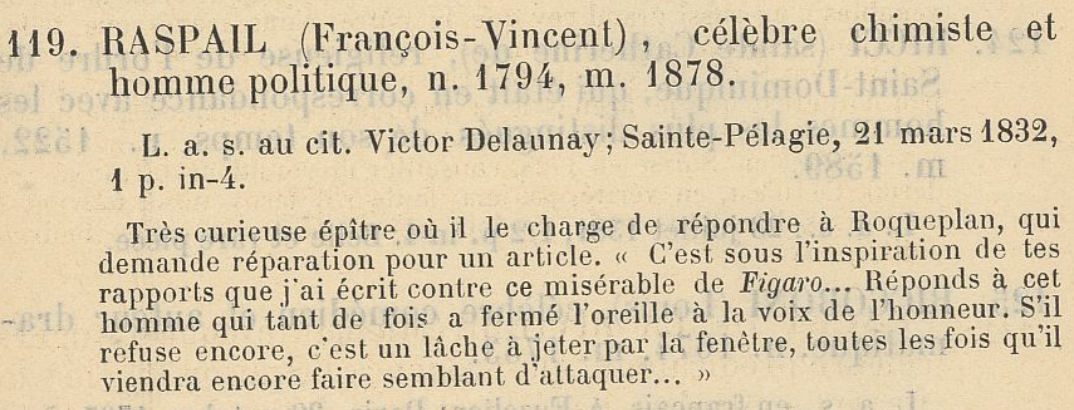
\includegraphics[width=\textwidth]{img/CAT_000441_e119}
	\caption{Une entrée de catalogue (\textit{Catalogue d'une précieuse collection de lettre autographes}, vente Étienne Charavay, 20 mai 1890)}
	\label{fig:catitem}
\end{figure}

Il apparaît donc que les catalogues de vente de manuscrits ont toujours une structure très rigide, aussi bien au niveau de l'ensemble du catalogue, que de la page et même de l'entrée. Des sauts de ligne marquent la différence entre les entrées et, dans les catalogues de vente aux enchères d'Étienne Charavay, des sauts de ligne distinguent également les différentes parties d'une entrée. D'autres caractères typographiques permettent d'établir des séparations supplémentaires entre les différentes informations présentes. Par exemple, le prénom est distinct du nom de famille à l'aide de parenthèses; une virgule distingue la description de l'auteur.ice de son nom. Enfin, à l'exception du paragraphe contenant des détails additionnels et du prix, tous les catalogues contiennent les mêmes informations. Il est donc possible de définir un modèle abstrait qui soit à même de représenter tous les catalogues (figure \ref{fig:catmodel}). Ce modèle peut servir de base pour structurer les données extraites des catalogues afin qu'elles soient manipulables.

\begin{figure}[h]
	\centering
	\tikz[scale=0.85,transform shape]{
		\node[base] (cat) at (0,0)%
		{Catalogue};
		\node[base] (intro) at (-5,-2)%
		{Titre et pages introductives};
		\node[base] (main) at (0,-2)%
		{Entrées de catalogues};
		\node[base] (conclu) at (5,-2)
		{Pages de fin};
		\node[base] (e1) at (-6.25,-4)%
		{Entrée 1};
		\node[base] (e2) at (-0,-4)%
		{Entrée 2};
		\node[base] (eN) at (6.25,-4)%
		{Entrée $n$};
		\node[base] (tname) at (-7.5,-6)%
		{
			Nom de l'auteur.ice
		};
		\node[expl] (exname) at (-7.5,-10)%
		{
			\begin{itemize}
				\item Nom de famille (usuel et nom de famille noble)
				\item Prénoms
				\item Titre de noblesse
			\end{itemize}
		};
		\node[base] (ttrait) at (-2.5,-6)%
		{
			Description de l'auteur.ice
		};
		\node[expl] (extrait) at (-2.5,-10)%
		{
			\begin{itemize}
				\item Occupation
				\item Date de naissance et de décès
				\item Parents ou proches illustres
			\end{itemize}
		};
		\node[base] (tdesc) at (2.5,-6)%
		{
			Description du manuscrit
		};
		\node[expl] (exdesc) at (2.5,-10)%
		{
			\begin{itemize}
				\item Type de document
				\item Dimensions
				\item Format
				\item Date
				\item Destinataire
			\end{itemize}
		};
		\node[base] (tnote) at (7.5,-6)%
		{Détails additionnels};
		\node[expl] (exnote) at (7.5,-10)%
		{
			\begin{itemize}
				\item Sujet du manuscrit
				\item Extrait du manuscrit
			\end{itemize}
		};
		\draw[arrow] (cat) -- (intro);
		\draw[arrow] (cat) -- (main);
		\draw[arrow] (cat) -- (conclu);
		\draw[arrow] (main) -- (e1);
		\draw[arrow] (main) -- (e2);
		\draw[arrow] (main) -- (eN);
		\draw[arrow] (e2) -- (tname);
		\draw[arrow] (e2) -- (ttrait);
		\draw[arrow] (e2) -- (tdesc);
		\draw[arrow] (e2) -- (tnote);
		\draw[arrow] (tname) -- (exname);
		\draw[arrow] (ttrait) -- (extrait);
		\draw[arrow] (tdesc) -- (exdesc);
		\draw[arrow] (tnote) -- (exnote);
	}
	\caption{Modèle d'un catalogue de vente de manuscrits}
	\label{fig:catmodel}
\end{figure}


\section{L'encodage des manuscrits en \xmltei{}}
\subsection{\textit{eXtensible Markup Language} et \textit{Text Encoding Initiative}: l'environnement technique pour encoder les catalogues}
Les possibilités pour encoder des données textuelles de façon numérique sont nombreuses, tant en termes de formats techniques que de standards qui pourraient être suivis pour encoder des documents. Pour représenter la complexité du texte, la structure de données arborescente du \xml{} est aujourd'hui privilégiée. Celle-ci est, de façon conventionnelle, considérée comme étant la meilleure manière de représenter un texte, qui serait lui-même composé en parties, chapitres, sections... Cette idée est notamment développée dans \textit{What is text, really?} (1990)\footcite{derose_what_1990}, article séminal sur la modélisation du texte sous forme d'arborescence co-écrit par Steven DeRose, l'un des concepteurs du \xml{} et se son ancêtre, le \texttt{SGML}. L'argumentaire développé par DeRose et al. porte sur l'idée que le discours sur le texte et ses représentations en dehors d'un environnement numérique sous-entendent déjà l'existence d'une structure arborescente pour le texte. Par exemple, un texte imprimé contient souvent une table des matières, organisée de façon hiérarchique; de la même manière, les manuels typographiques et autres chartes graphiques pour le texte définissent des règles de style qui s'appliquent à des ensembles, comme les blocs de citation, qui formerait un élément au sein d'une structure arborescente\footcite[p. 4]{derose_what_1990}. L'idée qu'un texte soit déjà une arborescence, en dehors de tout environnement technique, est bien sûr problématique et a été remise de nombreuses fois en question, comme nous le verrons. Cependant, elle est à la base d'une théorie centrale à la modélisation du texte: \gls{ohco}. Comme son nom l'indique, l'\gls{ohco} -- développée vers 1990 et défendue (entres autres) par DeRose, Durand, Mylonas et Renear -- revient à comprendre le texte comme une collection hiérarchisée d'unités linguistiques. Ces unités (page, partie, chapitre...) peuvent elles-mêmes en contenir d'autres. 

Ce modèle du texte est particulièrement intéressant d'un point de vue computationnel, surtout à la date où il a été élaboré, et c'est pour ces raisons que le modèle continue d'influencer la modélisation du texte aujourd'hui. Le principal avantage de l'\gls{ohco}, c'est qu'il permet de modéliser la structure du texte de façon indépendante de son apparence formelle (à l'inverse d'un éditeur de type \textit{LibreOffice} ou \textit{Microsoft Word}, où c'est la forme qui détermine la structure de données). Séparer la structure de l'apparence permet de réellement penser la modélisation du texte, c'est-à-dire sa représentation sous la forme d'une structure abstraite d'éléments imbriqués; la modélisation peut donc mettre en avant les aspects scientifiques du texte selon un vocabulaire codifié\footnote{
	Ce processus de modélisation, comme le remarquent Julia Flanders et Fotis Jannidis dans \textit{The shape of data in digital humanities}, n'est pas nécessairement dépendant d'une infrastructure informatique. L'édition critique, par exemple, est une forme de modélisation des textes et de la relation qu'ils entretiennent; elle s'appuie sur un système formel permettant de codifier l'information et de la représenter dans l'espace de façon synthétique\footcite[p. 3-4]{flanders_data_2019}.
}. Cette structuration non-formelle du texte est également garante d'interopérabilité, puisqu'elle peut s'appuyer sur des formats ouverts, là où de nombreux logiciels de traitement de texte sont propriétaires. En modélisant directement le texte, il est également possible de l'enrichir grâce à de nombreux éléments méta-textuels -- comme des notes ou des éléments de bibliographie -- et de distinguer ceux-ci du corps du texte\footcite[p. 11-13]{derose_what_1990}. DeRose, Durand, Mylonas et Renear envisagent déjà qu'un encodage conforme avec les principes de l'\gls{ohco} permettrait le traitement automatisé des documents, puisque dans ces formats la structure de données est explicite (contrairement aux logiciels de traitement de texte à interface graphique)\footcite[p. 17-18]{derose_what_1990}. Il existe de plus des systèmes de validation, pour garantir le respect d'un schéma \xml{} ou \texttt{SGML}; ensuite, ces documents encodés peuvent servir de bases de données d'où des informations peuvent être extraites et diffusées de façon automatique. Enfin, un document modélisé selon les principes de l'\gls{ohco} peut être transformé en de nombreux autres formats, y compris en une édition papier traditionnelle.

Le \xml{} est un format qui permet d'implémenter techniquement les principes de l'\gls{ohco} afin d'encoder des données brutes et des documents textuels. En \xml{}, les différents \enquote{objets linguistiques} doivent être encodés dans des éléments, dont le début est marqué par une balise ouvrante et la fin par une balise fermante. Par exemple, le nom d'une personne peut être encodée dans une balise \texttt{name}: \mintinline{xml}|<name>Virginia Woolf</name>|. Cet élément peut être complété par informations supplémentaires, contenues dans des attributs situés au niveau de la balise ouvrante, comme ici un identifiant: \mintinline{xml}|<name id="vw">Virginia| \mintinline{xml}|Woolf</name>|. Un élément peut être contenu dans un autre, ou en contenir d'autres; cependant, deux éléments ne doivent pas se chevaucher; tous les éléments ouverts demandent à être fermés. Enfin, dans un document \xml{}, tous les objets linguistiques doivent être contenus à l'intérieur d'un élément, qui est dit l'élément racine.

Cette structure définie par la spécification \xml{} ne précise pas les éléments qui sont autorisés; il est donc possible de réaliser un encodage sans s'aligner sur des standards. Cependant, pour permettre l'interopérabilité des documents et garantir des encodages plus qualitatifs, des standards se sont progressivement développés. Ceux-ci définissent un ensemble d'éléments qui peuvent être autorisés dans un document \xml{}, ainsi que la manière dont ces éléments peuvent être combinés pour former un document complet et valide. Ces standards sont souvent propres à des communautés scientifiques. Pour l'encodage du texte dans des projets de recherche, c'est la \texttt{Text Encoding Initiative} (\tei{}) qui domine. Ce projet, développé de façon communautaire par le \textit{TEI Consortium} depuis 1987 et à l'origine de Lou Burnard, vise à établir une sémantique commune pour le balisage de n'importe quel type de texte. La manière dont Burnard définit la \tei{} montre l'influence de l'\gls{ohco}: selon lui, le principe de ce standard est de modéliser le texte sous la forme d'un ensemble d'objets interconnectés à l'intérieur d'une structure qui soit représentative d'une lecture d'un texte\footcite[p. 108]{burnard_how_2019}. Le projet se dévelope comme une solution alternative à deux écoles de pensées qui dominaient le traitement computationnel du texte dans les années 1980. La première école considérait le texte comme un artefact physique (où c'est donc la structure formelle du document, y compris des pages, qui est signifiante). La deuxième développe une approche linguistique du texte: celui-ci est un phénomène du langage, fait de mots et de leur interrelation; dans ce cas, il n'importe pas de modéliser la structure globale d'un texte. L'approche de la \tei{} retient quelques aspects de ces deux approches et voit le texte comme une structure d'objets linguistiques, mais aussi comme une instance d'un modèle\footcite[§3]{burnard_search_2021}. Le deuxième aspect est important pour comprendre la spécificité de la \tei{} par rapport à d'autres standards d'encodage: il existe une différence entre le texte et le modèle utilisé pour encodé celui-ci. Un modèle est une spécification propre à un projet, faite à partir de la \tei{}, qui sert à représenter un corpus précis de documents. 

Pour structurer ces documents, la \tei{} définit un ensemble d'éléments, qui ont chacun une signification précise et auxquels un ensemble de contraintes peuvent être attachées: un élément ne peut être contenu que dans certains éléments, en contenir certains autres (ou aucun) et n'avoir que certains attributs. Les éléments sont définis avec une approche sémantique: une balise doit servir à expliciter la signification ou le rôle de l'objet linguistique qu'elle sert à encoder. Les éléments utilisés n'ont donc pas toujours d'équivalent formel qui serait identifiable dans un document physique. La définition de ces éléments est faite à partir de besoins de chercheurs, puisque les communautés d'utilisateur.ice.s sont libres de proposer la création de nouveaux éléments\footcite[p. 110]{burnard_how_2019}. Il s'ensuit que la \tei{} est particulièrement complexe et riche de possibilités pour une très grande variété de documents (manuscrits comme imprimés, éditions critiques, textes en vers ou en prose, pièces de théâtre ou encore transcription d'enregistrements sonores). En plus de l'encodage du texte, la \tei{} se distingue par l'importance qu'elle apporte aux métadonnées\footcite[p. 104]{burnard_how_2019}. Chaque document encodé contient un en-tête décrivant le document source ainsi que l'encodage numérique. Pour mettre en avant le rôle de la \tei{} comme \enquote{machine à générer des modèles}\footnote{\textit{machine for generating schemas}, \cite[§ 30]{burnard_what_2019}.}, ce standard permet également de créer un \enquote{méta-document} \xml{} qui permette de définir des modèles de données: le \gls{odd}. Ce document peut être qualifié de \enquote{méta}, puisqu'il contient des métadonnées relatives, non pas à un document, mais à un modèle pouvant être utilisé sur plusieurs documents. Il contient donc une documentation définissant les choix d'encodage pour un modèle; de plus, il contient une spécification technique qui peut servir à valider des documents encodés en suivant ce schéma (un document \tei{} n'est valide que si il se conforme à une \gls{odd}, et cette vérification peut être faite automatiquement). Une \gls{odd} peut contenir des modèles très complexes, puisque la spécification \tei{}, son schéma et sa documentation, sont encodés sous la forme d'une seule \gls{odd}. La \tei{} permet donc un encodage scientifique des documents, mais aussi la définition d'un modèle de données sur-mesure qui puisse être utilisé pour une variété de documents; grâce à l'accent mis sur la documentation et les métadonnées, il est possible de décrire précisément les documents d'origines, mais aussi la manière dont ils ont été encodés et pourquoi ces choix d'encodage ont été faits. C'est donc grâce à ce standard que les documents sont encodés.

\subsection{Encoder les catalogues en \tei{}}
Le schéma conçu pour encoder les catalogues du projet \mssktb{} ressemble, dans les grandes lignes, au modèle présenté en \ref{fig:catmodel}. Cependant, parce que le projet se concentre sur les manuscrits vendus dans les catalogues, une sélection a été fait dans l'édition pour se concentrer sur les items en vente. L'édition, présentée ci-dessous, a pour élément racine une balise \texttt{tei:TEI} (comme tous les documents suivant les principes de la \textit{Text Encoding Initiative}). Cet élément présente un identifiant \texttt{@xml:id} qui permet d'identifier le catalogue précisément. Cet identifiant est composé de \enquote{CAT\_} suivi d'une séries de chiffres, puisque les catalogues sont numérotés en quotation continue.

\subsubsection{Le \texttt{tei:teiHeader}}
Comme toute édition \tei{}, le schéma défini pour encoder les catalogues commence par un long \texttt{tei:teiHeader} contenant des métadonnées descriptives. Il est lui-même composé de plusieurs sous-éléments. 

Le premier est le \texttt{tei:fileDesc}, qui contient des informations portant sur l'édition numérique et sa source, le catalogue papier. Il contient notamment le titre du document (dans un \texttt{tei:titleStmt}) et des informations sur la publication du document électronique, comme la licence sous laquelle il est distribué (dans un \texttt{tei:publicationStmt}). Toujours dans le \texttt{tei:fileDesc} se trouve un \texttt{tei:sourceDesc} qui sert à décrire les catalogues papiers (exemple \ref{code:sourcedesc}). La description faite de ceux-ci est à plusieurs niveaux. D'abord est construite une notice bibliographique complète du catalogue, dans un \texttt{tei:bibl}. Cependant, ce n'est pas n'importe quel exemplaire de ces catalogues qui est encodé, mais un exemplaire précis. Celui-ci porte de nombreuses inscriptions manuscrites , puisque le commissaire priseur inscrit le prix des différents manuscrits vendus et le nom de leur acheteur.euse en face de l'item correspondant. En reprenant la typologie développée par l'ontologie de bibliothéconomie \gls{frbr}, les catalogues sont donc encodés comme manifestation plutôt que comme items\footcite[p. 28]{rondeau_du_noyer_encoder_2019}. Pour identifier spécifiquement l'exemplaire du catalogue encodé, la notice bibliographique est complétée d'un \texttt{tei:listWit} contenant un \texttt{tei:witness}, éléments généralement utilisés pour décrire les témoins d'une édition critique. Dans le \texttt{tei:witness}, le catalogue est décrit dans un \texttt{tei:msDesc}; celui-ci sert généralement à décrire les manuscrits, mais est ici utilisé puisque le document encodé est un unicum. Mais les catalogues de vente aux enchères sont publiés pour et existent en vertu de cette vente. Dans ce cas, le \texttt{tei:sourceDesc} est complété d'un \texttt{tei:listEvent} contenant un \texttt{tei:event} pour encoder des informations sur la vente. Celle-ci est notamment décrite avec sa date et son adresse ainsi que le nom des commissaires priseurs.
	
\begin{listing}[h]
	\begin{minted}{xml}
<sourceDesc>
	<bibl>
		<!-- description bibliographique du catalogue -->
	</bibl>
	<listEvent>
		<event>
			<!-- description de la vente -->
		</event>
	</listEvent>
	<listWit>
		<witness>
			<msDesc>
				<!-- description de l'exemplaire encodé -->
			</msDesc>
		</witness>
	</listWit>
</sourceDesc>
	\end{minted}
	\caption{Modèle de \texttt{tei:sourceDesc}}
	\label{code:sourcedesc}
\end{listing}
	
L'élément utilisé après le \texttt{tei:fileDesc} est un \texttt{tei:profileDesc}. Il sert uniquement à indiquer la langue dans laquelle le catalogue est encodé de façon normalisée, comme le montre l'exemple ci-dessous (\ref{code:profiledesc}).

\begin{listing}[h]
	\begin{minted}{xml}
<profileDesc>
	<langUsage>
		<language ident="fr"/>
	</langUsage>
</profileDesc>
	\end{minted}
	\caption{Usage du \texttt{tei:profileDesc}}
	\label{code:profiledesc}
\end{listing}

Le dernier élément présent dans le \texttt{tei:teiHeader} est le \texttt{tei:encodingDesc} (exemple\ref{code:encodingdesc}), qui permet de définir les normes suivies pour l'encodage d'un catalogue, et la manière dont un document a été encodé. Le premier élément contenu dans le \texttt{tei:encodingDesc} est un \texttt{tei:samplingDesc}. Celui-ci indique que l'intégralité du document n'a pas été encodée, mais seulement la liste des manuscrits en vente. Suit le \texttt{tei:appInfo}, qui permet d'indiquer les applications utilisées pour produire le présent encodage. Au cours du projet, trois applications (\textit{Transkribus, eScriptorium} et \textit{GROBID-Dictionnaries}) ont été utilisées; deux \texttt{tei:application} sont donc utilisés, l'un pour indiquer l'utilisation de \textit{GROBID-Dictionnaries} et l'autre pour mentionner la plateforme de transcription utilisée (\textit{Transkribus} ou \textit{eScriptorium}). C'est encore dans le \texttt{tei:encodingDesc} que sont définis les termes spécifiques au projet qui sont utilisés dans les catalogues et qui pourraient ne pas être compris. Les termes sont classifés en \texttt{tei:taxonomy} (avec une taxonomie par sujet, contenues dans un \texttt{tei:classDecl}). Chaque terme à définir est conteny dans un \texttt{tei:category}. Un attribut \texttt{@xml:id} pointe vers le terme à définir; la définition se trouve dans un élément \texttt{tei:catDesc} qui est incluse dans l'élément précédent.

\begin{listing}[h]
	\begin{minted}{xml}
<encodingDesc>
	<samplingDesc>
		<!-- description des pages de catalogues conservées -->
	</samplingDesc>
	<appInfo>
		<!-- applications utilisées pour la production du document -->
	</appInfo>
	<classDecl>
		<taxonomy xml:id="identifiant de la taxonomie">
			<category xml:id="terme à définir">
				<catDesc>
					<!-- définition du terme -->
				</catDesc>
			</category>
		</taxonomy>
	</classDecl>
</encodingDesc>
	\end{minted}
	\caption{Usage du \texttt{tei:encodingDesc}}
	\label{code:encodingdesc}
\end{listing}

Ainsi, le \texttt{tei:teiHeader} contient des données permettant de décrire le document original d'une façon bibliographique ainsi que d'identifier un exemplaire précis utilisé pour l'encodage. Est également décrite l'édition numérique; le vocabulaire spécifique qui y est utilisé ainsi que les outils techniques utilisés pour produire le document numérique sont indiqués. Ce \texttt{tei:teiHeader} remplace la page de titre qui est présente dans les catalogues papier, puisque toutes les informations présentes sur cette page se retrouvent dans l'en-tête du document numérique.

\subsubsection{Encoder le corps des catalogues dans le \texttt{tei:text}}
En comparaison avec l'en-tête, le corps des catalogues est relativement simple et suit de très prêt le modèle abstrait présenté en \ref{fig:catmodel}. Le \texttt{tei:text} sert à accueillir l'intégralité d'un document encodé; il peut contenir un \texttt{tei:front} (pour l'avant-propos, la préface ou tout autre élément ne faisant pas directement partie du document), un \texttt{tei:body} qui contient le corps du document et un \texttt{tei:back} qui contient tout ce qui vient après le corps. Dans le projet \mssktb{}, seules les entrées des documents sont encodées; l'élément \texttt{tei:body} est donc le seul utilisé. Dans les catalogues imprimés, les items en vente se succèdent sans autre forme de hiérarchie. L'ensemble des documents est donc contenue dans un \texttt{tei:list} (exemple \ref{code:body}).

\begin{listing}[h]
	\begin{minted}{xml}
<text>
	<body>
		<list>
			<item>
				<!-- première entrée de catalogue -->
			</item>
			<item>
				<!-- deuxième entrée -->
			</item>
			<!-- ... -->
		</list>
	</body>
</text>
	\end{minted}
	\caption{Modèle du \texttt{tei:text}}
	\label{code:body}
\end{listing}

Chaque item en vente a la même structure (visible en \ref{code:teiitem}). Il est contenu dans un élément \texttt{tei:item}. Celui-ci a deux attributs obligatoires: \texttt{@n} qui contient le numéro de l'entrée dans le catalogue ainsi qu'un indentifiant unique \texttt{@xml:id} pour cet item. L'identifiant est composé du \texttt{@xml:id} du catalogue suivi de \texttt{e\_} (pour \textit{entry}) et du numéro de l'entrée. Le \texttt{tei:item} contient ensuite un \texttt{tei:num} qui là encore indique le numéro de l'entrée de catalogue. Ensuite, un \texttt{tei:name} est utilisé pour définir le nom indiqué dans un catalogue. Celui-ci est souvent celui de l'auteur.ice du document en vente, mais ce n'est pas toujours le cas. C'est pourquoi un attribut \texttt{@type} est utilisé, qui peut prendre pour valeurs \textit{author} ou \textit{other}, afin de caractériser le texte contenu par l'élément. Ensuite, un \texttt{tei:trait} est utilisé pour contenir la description de l'auteur.ice du document. Lorsque cet élément optionnel est utilisé, le texte est contenu dans un paragraphe \texttt{tei:p}. La description de la pièce en vente est contenue dans un \texttt{tei:desc}. Le texte de celle-ci est le même que celui des catalogues, mais il est enrichi au cours de la chaîne de traitement d'éléments qui permettent de cibler les différentes informations présentes et de les normaliser. Un \texttt{tei:date} sert notamment à indiquer la date; deux \texttt{tei:measure} sont utilisés, le premier pour indiqué la longueur du document (en pages, le plus souvent) et le second pour indiquer son format (\textit{in-octo, in-quatro}...). Si un item a un prix, un élément \texttt{tei:measure} est utilisé pour le contenir. La monnaie dans laquelle il est vendu est indiquée dans un attribut \texttt{@unit}. La description de l'élément est enfin complétée de deux éléments additionnels: un \texttt{tei:note} contenant les notes supplémentaires sur l'item et un \texttt{tei:add} qui n'est utilisé que pour les ventes aux enchères. Ce dernier permet d'indiquer le prix auquel un manuscrit a été vendu lors d'une vente aux enchères, information qui n'est pas présente dans l'imprimé mais souvent rajoutée à la main par le commissaire priseur.

\begin{listing}[h]
	\inputminted{xml}{code/tei_item.xml}
	\caption{Exemple d'entrée de catalogue encodée dans un \texttt{tei:item}}
	\label{code:teiitem}
\end{listing}


\subsection{L'encodage en \tei{} comme lecture du texte}
L'encodage des catalogues de vente de manuscrit vise à garder le lien avec l'exemplaire originel (en utilisant les \texttt{tei:witness} et \texttt{tei:msDesc}). Cependant, un encodage numérique ne peut représenter toute la richesse d'informations qui sont contenues dans un document physique. Une certaine perte d'information est nécessaire, et il peut être intéressant de situer ce qui est conservé et ce qui est perdu dans la transcription. Cela peut notamment permettre de mieux comprendre le matériau de travail utilisé dans les chaînes de traitement présentées dans les parties suivantes.

\subsubsection{L'encodage comme sélection}
Dire qu'une édition numérique ne soit pas un double transparent d'un original est bien sûr un fait évident; c'est d'ailleurs pourquoi la \tei{} demande des encodeur.euse.s d'expliciter le plus possible la sémantique utilisée dans un document, à l'intérieur d'un \texttt{tei:teiHeader}\footcite[p. 104]{burnard_how_2019}. Mais des travaux de recherche se sont également développés pour mieux préciser ce qui est conservé et ce qui est perdu dans un processus d'encodage. Le philologue allemand Patrick Sahle a notamment élaboré un cadre de pensée pour mieux comprendre une édition numérique. Il met en avant que le processus d'édition n'est pas la traduction d'un document physique en sa version numérique, mais une transcription du contenu et de la signification d'un texte dans une forme numérique; cette transcription se fait au delà de la \enquote{médialité} des documents: le contenu du document est perçu, dans une large mesure, comme étant distinct de sa forme et comme étant indépendant d'un médium physique\footcite{sahle_digital_2016}. L'édition numérique vient donc avec une forme d'abstraction, d'éloignement de la matérialité du document vers l'idée que le texte est un contenu, une donnée qui peut être isolée de l'objet physique; c'est ce contenu qui est encodé dans une édition numérique. Celles-ci ne peuvent en effet pas intégrer, par exemple, des images, et les descriptions de zones graphiques sont souvent très succintes -- lorsqu'elles sont retranscrites, ce qui n'est pas le cas dans les catalogues encodés. Pour mieux caractériser la spécificité de l'encodage numérique, il est importante mieux cerner quelles sont les possibles significations contenues dans un texte, afin de mieux comprendre ce qui est transmissible et ce qui est perdu dans un texte. 

Pour Peter Sahle, un texte est pluriel, et cette pluralité peut être représentée sous la forme d'une roue (visible en \ref{fig:wheeloftext} à partir d'une présentation de l'auteur datant de 2016\footcite[p. 21]{sahle_what_2016}). Cette roue est un bon point de départ pour mieux comprendre ce qui est perdu dans une édition numérique. Idéalement, une édition \tei{} doit chercher à représenter le texte \enquote{comme idée et comme contenu}, c'est-à-dire à être le plus fidèle possible à un texte; se pose alors la question de ce qui fait \enquote{l'idée} ou \enquote{la nature} d'un texte, idée du texte qui est distincte du document, qui est une occurrence d'un texte. Cette question, d'ordre plutôt ontologique, ne peut être répondue aisément, et encore moins dans le cadre de ce mémoire. Cependant, les différents aspects de la roue de Peter Sahle permettent de mieux situer les outils disponibles pour retranscrire \enquote{l'idée} d'un texte dans une édition numérique. Celle-ci s'appuie sur du texte encodé, et non sur de l'image; cela rend d'office la représentation du \enquote{texte comme document physique} et comme \enquote{objet visuel} difficile, bien que la \tei{} permette la description des caractéristiques physiques. Le \enquote{texte comme ensemble de caractères}, c'est-à-dire le texte comme \textit{écriture}, est déjà plus représentable: la \tei{} permet la représentation d'une très grande variété de caractères et dispose d'éléments pour indiquer la présence de corrections, de reprises ou d'autres particularités graphiques. Une transcription perd cependant nécessairement l'image des caractères écrits ou imprimés (il est possible de décrire une fonte, mais pas d'écrire le texte avec cette fonte dans une édition numérique). Ce que la \tei{} permet réellement, par contre, c'est la représentation du texte comme, justement, un texte (et non comme un objet physique). La transcription transmet la \enquote{structure rhétorique} du texte; elle conserve et structure les objets linguistiques dont un texte est fait. L'édition numérique des catalogues est donc une étape utile, puisqu'elle permet le stockage de l'information contenue dans le texte et le traitement automatisé ultérieur des catalogues. Cependant, les caractéristiques physiques sont perdues; les catalogues encodés perdent donc toute valeur par exemple, pour une faire une étude des spécificités de la typographie du \scl{XIX}.

\begin{figure}[h]
	\centering
	\tikz{
		\node[name=c, circle,draw=plum,fill=lightmauve,minimum width=5cm, text width=7cm] (c) at (0,0) %
			{\begin{center}\textbf{Différentes significations \\ du texte}\end{center}};
		\foreach \a / \p / \t in {
			north/above/Texte comme idée et comme contenu,
			north east/right/Texte comme œuvre et structure rhétorique,
			south east/right/Texte comme objet linguistique et comme suite de mots,
			south/below/Texte comme ensemble de caractères avec particularités graphiques,
			south west/left/Texte comme document physique individuel,
			north west/left/Texte comme objet visuel et comme signe complexe
		}
		\draw[shift=(c.\a)] plot[mark=*] coordinates{(0,0)} node[\p=0.5cm,text width=4cm] {\t};
	}
	\caption{Les différentes signification d'un texte selon P. Sahle (2016)}
	\label{fig:wheeloftext}
\end{figure}

\subsubsection{Forme du texte, lecture et généricité}
En perdant les caractéristiques physiques de la page, et de la manière dont les informations s'organisent à l'intérieur d'un document physique, c'est également la lecture du texte encodé qui est modifiée. Pour aborder la question de la lecture d'une édition numérique, il peut être intéressant de faire un détour par la théorie du genre littéraire. Selon John Frow\footcite{frow_genre_2006}, le genre doit être compris, non pas comme une définition rigide, mais comme une action symbolique qui organise des textes et les met en interrelation; le genre créée des réseaux de textes, et les textes, en retour, se positionnent vis à vis d'un champ de genres. Dès lors, le genre permet de sortir d'une analyse \enquote{isolée} du texte pour comprendre comment les textes fonctionnent de façon intertextuelle et référentielle; la signification du texte existe dans un champ social\footcite[p. 2, 10]{frow_genre_2006}. Le genre sert de médiation pour le texte\footcite[p. 14]{frow_genre_2006}: il permet aux lecteur.ice.s de comprendre dans quel contexte s'inscrit un texte. Du côté des lecteur.ice.s, il construit un ensemble d'attentes, et des formes de lecture spécifiques qui seront utilisées pour appréhender et comprendre un texte; du côté du texte, il crée un ensemble de significations et de valeurs qui seront implicitement présentes dans le texte\footcite[p. 83-87]{frow_genre_2006}. Le genre, dans l'approche de Frow, a une acception bien plus large que celle qui est habituellement utilisée: le roman policier est un genre, mais un journal d'informations fonctionne aussi comme un genre (il construit des horizons d'attentes spécifiques pour le public et prépare à certaines formes de lecture); de même, le catalogue de vente peut être considéré comme un genre à part entière. Le catalogue, en tant que genre, encadre des descriptions de manuscrit et les fait rentrer dans un contexte marchand; il vient avec le développement de formes de descriptions particulières des manuscrits, et vient avec un système de valeurs particulier, marqué notamment par l'importance des \enquote{hommes illustres} et autres figures historiques importantes. Le genre modèle donc l'interprétation; en quoi cela impacte-t-il une édition numérique? Le problème est posé par l'abandon des caractéristiques physiques du texte. En effet, un genre fonctionne très largement par le fait qu'un document physique présente les particularités physiques attendues d'un texte: le genre existe par une structure formelle\footcite[p. 19]{frow_genre_2006}. La disposition d'un poème en vers sur une page, par exemple, est un signe visuel qui indique que le texte est un poème, et non une pièce de théâtre. Mais les caractéristiques formelles du genre peuvent s'exprimer à l'extérieur du texte lui-même. Par exemple, la couverture d'un roman noir est très souvent porteuse de tropes du genre (surtout dans les collections anciennes). Dans le cas d'un catalogue de vente, la disposition des items en vente sur la page est signifiante, de même que, dans le cas de la \textit{Revue des autographes}, la présente d'articles et de réclames en plus des items en vente eux-mêmes. Prendre en compte la généricité du texte amène à constater un problème inhérent à toute édition numérique. En effet, la généricité s'appuie sur des tropes, qui peuvent être textuels, mais qui sont tout autant visuels: le genre dans lequel un texte s'inscrit peut être reconnu sans nécessairement avoir besoin de lire le texte. Or, une édition numérique n'a, par définition, pas de forme (puisque une édition \xml{} vise à représenter la structure du texte, alors que sa forme sera le fait d'une transformation ultérieure). Cette absence de forme du texte interrompt, ou empêche, l'utilisation des mécanismes de lecture qui s'appuient sur les aspects formels du texte, et peut donc limiter les interprétations qui peuvent être faites de celui-ci.

\subsubsection{Critiques de l'OHCO}
Cette critique de l'encodage numérique se repose sur son absence de propriétés formelles, pourtant inhérentes à la production du sens d'un texte (ce qui est d'autant plus vrai pour les manuscrits et documents illustrés). Elle revient à mettre en avant une conception du texte comme artefact physique, une école de pensée que Burnard et al. opposent à la compréhension du texte défendue par la \tei{} (le texte comme instance d'un schéma)\footcite[§ 3]{burnard_search_2021}. Mais l'absence de propriétés formelles du texte n'est pas la seule critique qui peut être faite à la \tei{}, ni au format \xml{} utilisé. La théorie de l'\gls{ohco}, à la base de celui-ci, semble critiquable: comment peut-on définir une forme \enquote{implicite} à tous les textes, une structure unique pouvant contenir n'importe quel document textuel, de toutes les époques possibles et de différentes régions du globe? C'est justement parce que les prétentions de l'\gls{ohco} sont trop grandes que cette théorie a été l'objet de débats dès sa création, et a connu de nombreuses reformulations. Il est important de remarquer que les critiques de cette théories sont faites par David Durand, Elli Mylonas et Allen Renear, trois des quatres auteur.ice.s de l'article séminal \textit{What is text, really}\footcite{derose_what_1990}. En effet, dès 1996, les chercheur.euse.s publient une réfutation de leur théorie originelle dans l'article \textit{Refining our notion of what text really is: the problem of overlapping hierarchies}\footnote{\enquote{Redéfinir notre notion de ce qui fait le texte: le problème des hiérarchies multiples}}\footcite{renear_refining_1996}. Dans cet article sont énoncés non pas un, mais trois \gls{ohco}. La première version de cette théorie correspond à celle du premier article: un texte est une collection ordonnée d'objets. La première et la deuxième reformulation de cette théorie supposent la possible coexistence entre plusieurs représentations d'un même texte. Un texte n'est pas en lui-même une collection d'objets. Cependant, un texte peut être interprété comme une collection d'objets: une analyse, propre à un domaine académique, détermine une représentation d'un texte sous la forme d'une collection ordonnée d'objets\footcite{renear_refining_1996}. L'acceptation progressive de cette pluralité permet de mettre l'accent sur les choix d'encodage possibles dans la modélisation d'un texte, et donne de l'importance à celle-ci, qui représente un processus intellectuel. La modélisation du texte n'est pas le texte lui-même, mais une lecture de celui-ci. Ces reformulations successives n'arrivent cependant pas à régler le problème central du \xml{}: le fait qu'il n'autorise qu'une hiérarchie unique pour un texte. Il n'est pas possible de combiner deux hiérarchies différentes qui pourraient coexister au sein d'un même texte. On ne peut pas structurer un texte encodé par page et par paragraphe -- ou par ligne et par phrase --, puisqu'il risque d'y avoir des paragraphes qui s'étendent sur plusieurs pages. Il est également impossible de structurer le texte sous forme non hiérarchique, ou de représenter deux éléments cooccurents (c'est-à-dire, deux éléments qui, dans un document, apparaissent au même point du texte, sans que l'un ne soit placé avant l'autre)\footcite{bleeker_texts_2021}. Ce dernier problème est de circonstance dans le projet \mssktb{}, où des notes manuscrites sont faites par le commissaire priseur pour indiquer le prix de vente d'un item sur une page en face ce celui-ci. Les catalogues étant encodés en utilisant une structure hiérarchique, ces notes sont reportées dans des \texttt{tei:add} à l'intérieur des \texttt{tei:item} contenant l'entrée de catalogue. Cela positionne la note manuscrite à l'intérieur de l'entrée, ce qui dans les faits n'est pas le cas: la note est au même niveau que l'entrée, sans qu'il n'y ait de hiérarchie entre les deux éléments. Il n'est cependant pas possible en \xml{} de représenter ce genre de cas de figure. C'est pourquoi de nombreuses syntaxes alternatives se sont développées, dont le très récent \texttt{TAGML}, langage à balises permettant l'encodage de structures non-hiérarchiques ou encore de hiérarchies multiples: dans ce langage, le texte est représenté sous la forme d'un graphe, c'est-à-dire d'un réseau d'éléments connectés entre eux\footcite{bleeker_texts_2021}.

Malgré les problématiques inhérentes à l'usage du \xml{} qui ont été évoquées ici, force est de constater que ce format, avec l'usage de la \tei{}, est devenu incontournable dans l'encodage du texte. Quelques syntaxes alternatives sont développées, comme le \texttt{TAGML}, ou auparavant le \texttt{LMNL} qui visait lui aussi à résoudre le problème des hiérarchies multiples. Cependant, ces syntaxes n'ont pour l'instant jamais dépassé le stade d'objet expérimental. Malgré tous ses défauts, le \xml{} est, pour l'instant, un incontournable dans l'encodage du texte dans un projet d'édition numérique. Il suffisamment utilisé pour que des outils se soient développés pour le traiter, le manipuler et le transformer, ce qui en fait un format particulièrement utile comme base à une chaîne de traitement telle que celle de \mssktb{}. De plus, ce format est un standard du \gls{w3c}, l'instance de normalisation des technologies du Web. Ce format est donc un standard d'échange sur le Web, et c'est pourquoi il sera utilisé dans la conception d'une application Web qui diffuse les données de \mssktb{} de façon automatisée, présentée en troisième partie de ce mémoire.

\subsection{En conclusion}
Dans cette partie ont été présentés les documents sources du projet \mssktb{}, les catalogues de vente. La structure des catalogues, par nature répétitive, peut servir à mettre au point un modèle abstrait, pour représenter chaque document sous la forme d'une arborescence. Ce modèle abstrait a été ensuite explicité, afin d'arriver à l'encodage des catalogues de vente de manuscrits en \xmltei{}. Les choix d'encodage suivis dans l'édition numérique des catalogues vise à mettre en avant la structure implicitement présente dans ces documents. Expliciter cette structure, faite d'une suite d'items en vente décrits de façon toujours analogue, est un processus technique et intellectuel à la base de l'intégralité de la chaîne de traitement mise au point par \mssktb{}. En effet, un document structuré de façon aussi précise que le sont les catalogues peut être manipulé avec beaucoup d'aisance. Grâce à l'utilisation de la \tei{}, il est possible de ne traiter qu'un seul élément du document, comme le \tname{}. Le fait qu'un catalogue soit, par nature, semi-structuré permet de manipuler le contenu de cet élément avec des méthodes particulières, comme cela est montré dans la partie suivante. En effet, il devient possible de développer une chaîne de traitement qui s'appuie sur l'organisation répétitive des informations à l'intérieur d'un même élément pour extraire et manipuler des données.

Une dernière spécificité de l'édition numérique reste à présenter; celle-ci est, selon Peter Sahle, un processus, contrairement à l'objet fini qu'était une édition papier\footcite{sahle_digital_2016} -- une édition numérique est faite pour être reprise, modifiée et augmentée. Cette idée est centrale dans le projet \ktb{}, où l'ensemble de la chaîne de traitement est correspond à un enrichissement progressif des catalogues encodés et en une transformation de ceux-ci vers de nouveaux formats. C'est cette éditorialisation continue qui est présentée dans la deuxième et troisième parties de ce mémoire.